\documentclass[
10pt, % Main document font size
a4paper, % Paper type, use 'letterpaper' for US Letter paper
oneside, % One page layout (no page indentation)
%twoside, % Two page layout (page indentation for binding and different headers)
%headinclude,footinclude, % Extra spacing for the header and footer
%BCOR5mm, % Binding correction
%]{scrartcl}
]{article}
\usepackage{setspace}
\usepackage{longtable}
\usepackage{graphicx}
\usepackage[margin=1in]{geometry}
\usepackage{pdflscape}
%\usepackage[cm]{fullpage}
\doublespacing

\title{\normalfont{Molecular standardization}}

\begin{document}

\maketitle

The molecular standardization processes of ChemAxon's Standardizer and the Open Source library MolVS have been evaluated 
on a test suit of 35 compounds containing tautomers, mesomers and functional groups that are often represented differently. 
The 35 compounds are represented in multiple forms that, from a chemoinformatic perspective, should ideally be transformed 
into the same representation by the standardization process. 
However, the standardization process in Standardizer is not intended to transform into one canonical tautomer, but 
produces so called normal canonical tautomers where the normal canonical tautomer is selected from from subsets of 
tautomers considered interchangeable under physiological conditions. 

For each method a table is produced showing the input and output structures as drawn by RDKit for the different forms.
The table also displays two fingerprint similarities between all pairs of output structures. If the standardization 
is successful the fingerprints should be identical. Furthermore, the set of 177 RDKit descriptors is calculated 
for each output structure and the number of differing descriptors is reported for each pair of output structures.


%\section{Results Summary}
%ChemAxon's Standardizer fails to identify the different forms of 14 out of the 35 structures as similar, while MolVS fails 
%for 3 structures. The failures of MolVS are all for certain functional groups, nitro, phosphine and diazo, while 
%Standardizer fails in the canonicalization of 9 tautomers, as well as for 5 functional groups. 

%As shown in the tables below, most of the standardization failures result in significant loss of fingerprint similarity 
%and a large number of RDKit descriptors with different values. Hence, the failures will have an impact on the results of 
%chemoinformatic analysis. 


\section{Standardization with ChemAxon Standardizer }

The ChemAxon standardizer was used with 7 actions, applied in the following order, together with the set of transformations defined in the GUI:
\begin{itemize} 
\item removesolvents
\item stripsalts 
\item removefragment:method=keeplargest
\item mesomerize
\item tautomerize
\item neutralize
\item transformations
\item dearomatize
\end{itemize} 
%Two out of the failures to transform functional groups (Idx 7 and 35) originates from RDKit being unable to accept the valence of the structures 
%returned by Standardizer. The output structure of molecule 7 is displayed below. 
%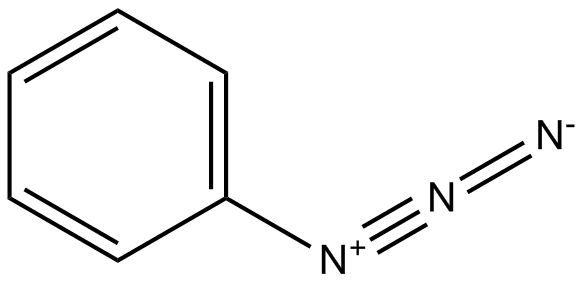
\includegraphics[scale=0.4]{azideCAout.png}
	

\begin{landscape}
\begin{longtable}{|l|l|l|l|l|l|l|}
\hline
Idx & Name & Structure In and Out & Comment & TanTop & DiceMorgan & No. of DescDiff\\
\hline
1 & clopidol & 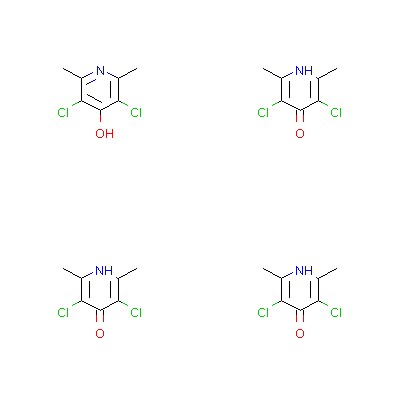
\includegraphics[scale=0.6]{clopidolCA.png} & & [1.0]& [1.0] & [0] \\
\hline
2 & phthalimide & 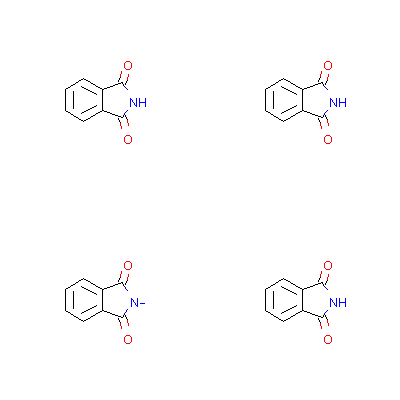
\includegraphics[scale=0.6]{phthalimideCA.png} & & [1.0]& [1.0] & [0] \\
\hline
3 & Viagra & 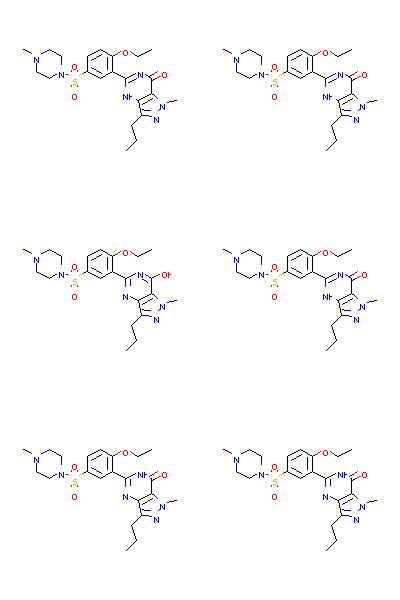
\includegraphics[scale=0.6]{ViagraCA.png} & & [1.0, 1.0, 1.0]& [1.0, 0.91, 0.91] & [1, 21, 21] \\
\hline
4 & quatAmMesomer & 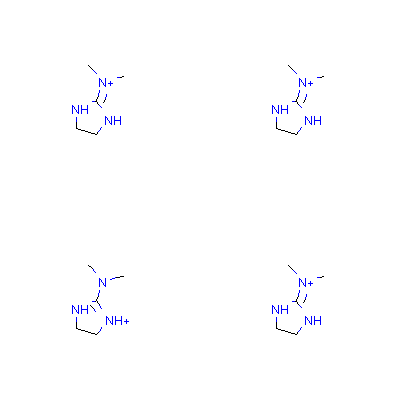
\includegraphics[scale=0.6]{quatAmMesomerCA.png} & & [1.0]& [1.0] & [0] \\
\hline
5 & pyridinol & 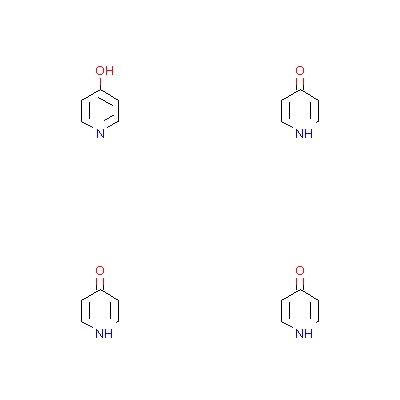
\includegraphics[scale=0.6]{pyridinolCA.png} & & [1.0]& [1.0] & [0] \\
\hline
6 & quatAmMesomer4 & 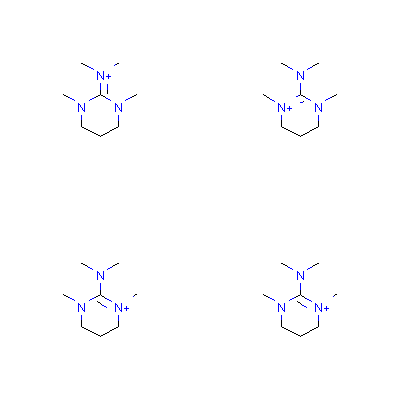
\includegraphics[scale=0.6]{quatAmMesomer4CA.png} & & [1.0]& [1.0] & [1] \\
\hline
7 & azide & 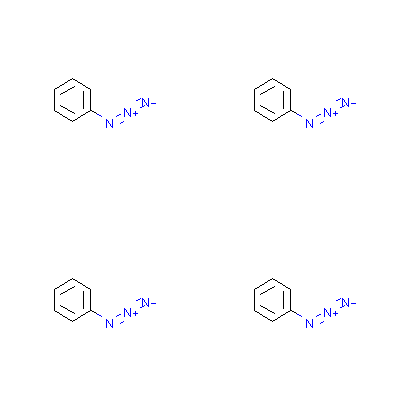
\includegraphics[scale=0.6]{azideCA.png} & & [1.0]& [1.0] & [0] \\
\hline
8 & triazinol & 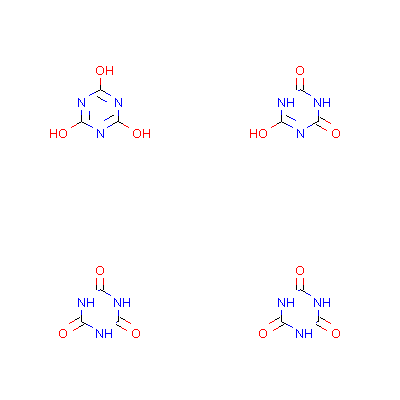
\includegraphics[scale=0.6]{triazinolCA.png} & & [0.58]& [0.54] & [50] \\
\hline
9 & phosphate & 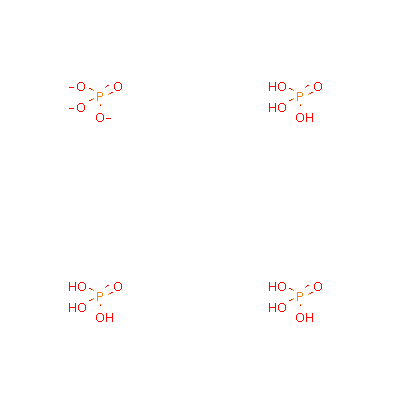
\includegraphics[scale=0.6]{phosphateCA.png} & & [1.0]& [1.0] & [0] \\
\hline
10 & Propenol & 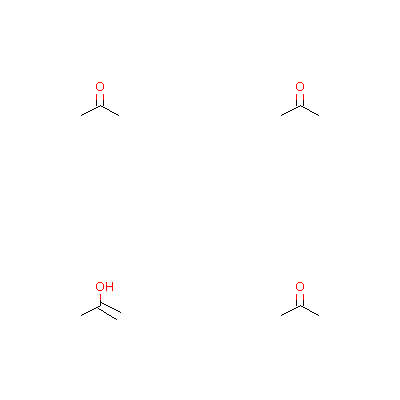
\includegraphics[scale=0.6]{PropenolCA.png} & & [1.0]& [1.0] & [0] \\
\hline
11 & phosphine & 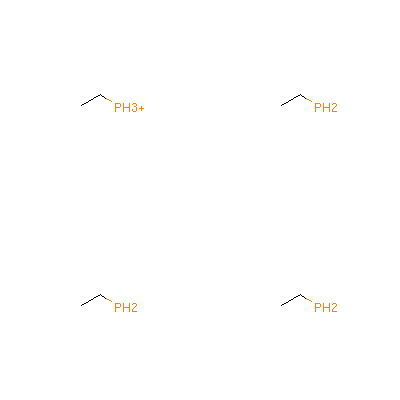
\includegraphics[scale=0.6]{phosphineCA.png} & & [1.0]& [1.0] & [0] \\
\hline
12 & cicletanine & 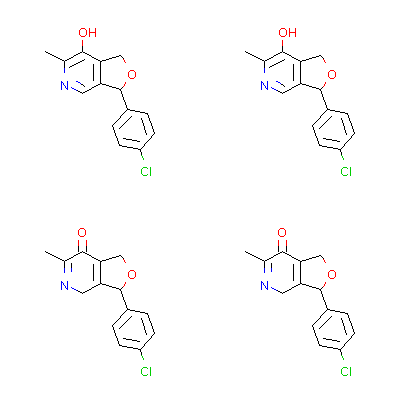
\includegraphics[scale=0.6]{cicletanineCA.png} & & [0.3]& [0.67] & [76] \\
\hline
13 & propaneAcid & 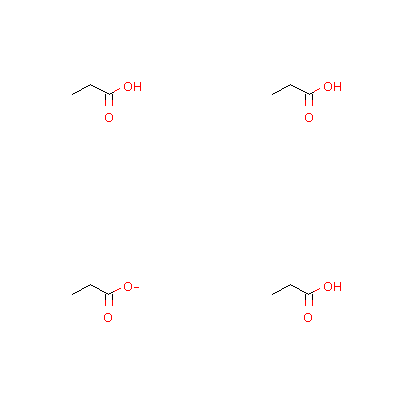
\includegraphics[scale=0.6]{propaneAcidCA.png} & & [1.0]& [1.0] & [0] \\
\hline
14 & imidazole & 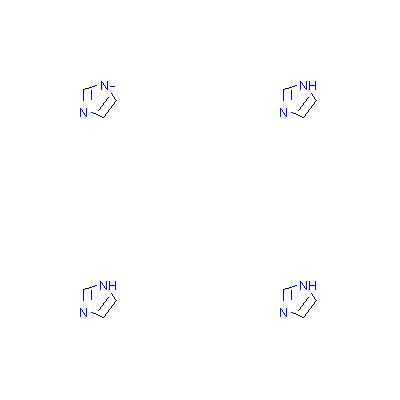
\includegraphics[scale=0.6]{imidazoleCA.png} & & [1.0]& [1.0] & [0] \\
\hline
15 & enamine & 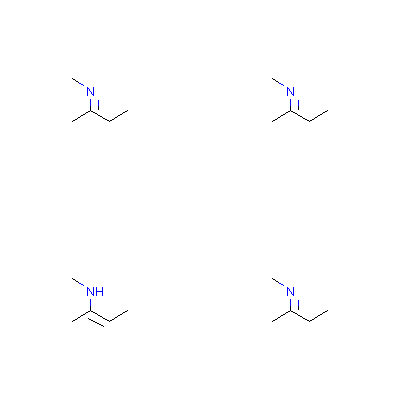
\includegraphics[scale=0.6]{enamineCA.png} & & [1.0]& [1.0] & [0] \\
\hline
16 & sulfoxide & 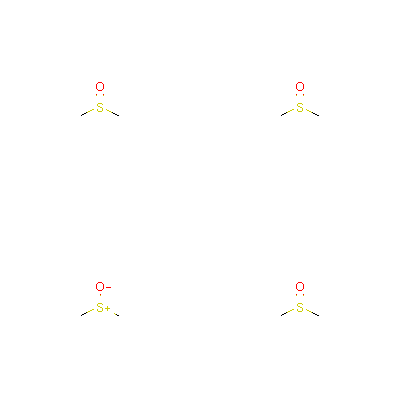
\includegraphics[scale=0.6]{sulfoxideCA.png} & & [1.0]& [1.0] & [0] \\
\hline
17 & sulfonamide & 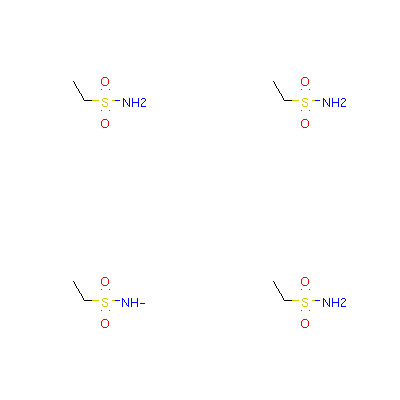
\includegraphics[scale=0.6]{sulfonamideCA.png} & & [1.0]& [1.0] & [0] \\
\hline
18 & tiouracil & 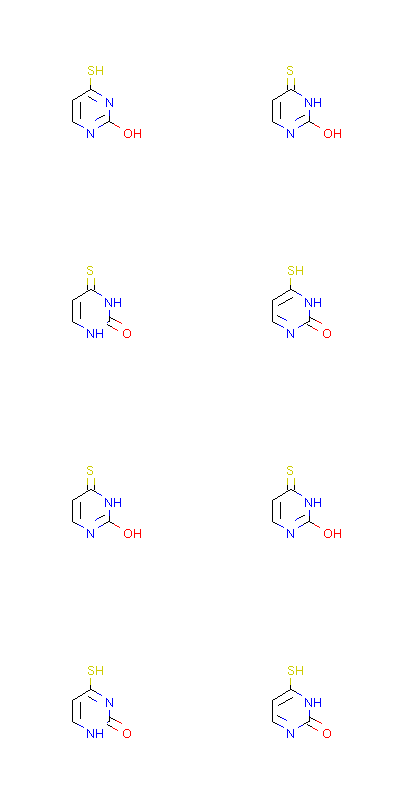
\includegraphics[scale=0.6]{tiouracilCA.png} & & [0.35, 1.0, 0.35, 0.35, 1.0, 0.35]& [0.5, 1.0, 0.5, 0.5, 1.0, 0.5] & [54, 0, 54, 54, 0, 54] \\
\hline
19 & quatAmMesomer2 & 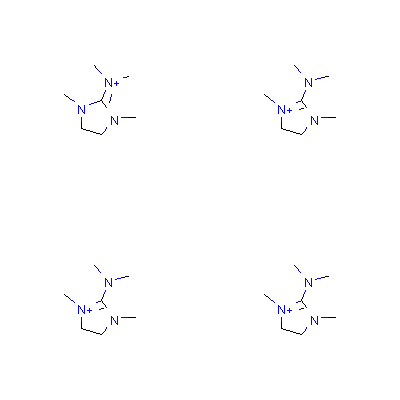
\includegraphics[scale=0.6]{quatAmMesomer2CA.png} & & [1.0]& [1.0] & [0] \\
\hline
20 & nitro & 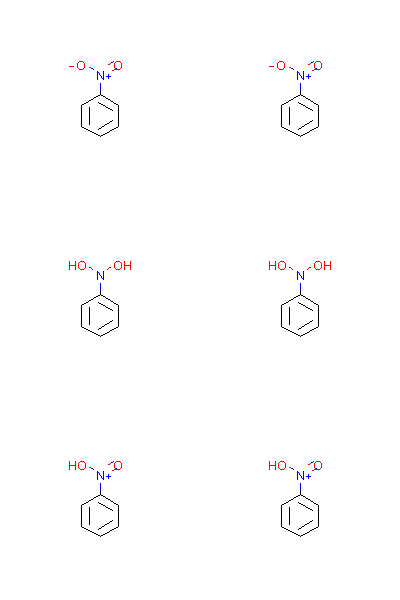
\includegraphics[scale=0.6]{nitroCA.png} & & [0.67, 1.0, 0.67]& [0.56, 0.8, 0.6] & [58, 43, 56] \\
\hline
21 & 107and108and109 & 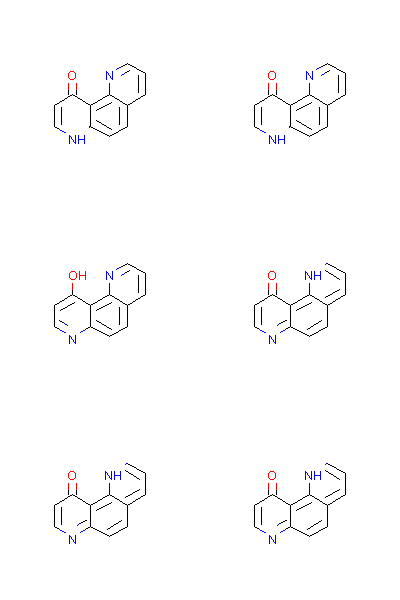
\includegraphics[scale=0.6]{107and108and109CA.png} & & [1.0, 1.0, 1.0]& [0.7, 0.7, 1.0] & [17, 17, 0] \\
\hline
22 & aminopyrimidine & 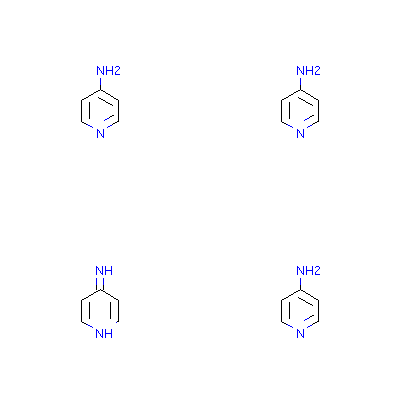
\includegraphics[scale=0.6]{aminopyrimidineCA.png} & & [1.0]& [1.0] & [0] \\
\hline
23 & 105and106 & 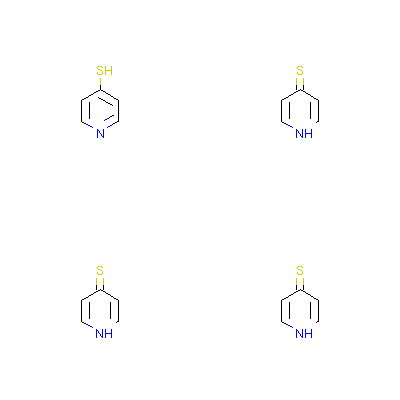
\includegraphics[scale=0.6]{105and106CA.png} & & [1.0]& [1.0] & [0] \\
\hline
24 & Rhodamine & 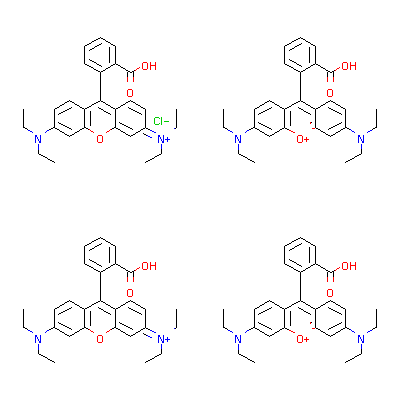
\includegraphics[scale=0.6]{RhodamineCA.png} & & [1.0]& [1.0] & [0] \\
\hline
25 & sulfon & 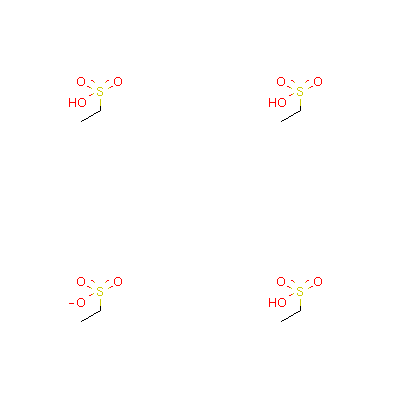
\includegraphics[scale=0.6]{sulfonCA.png} & & [1.0]& [1.0] & [0] \\
\hline
26 & triazine & 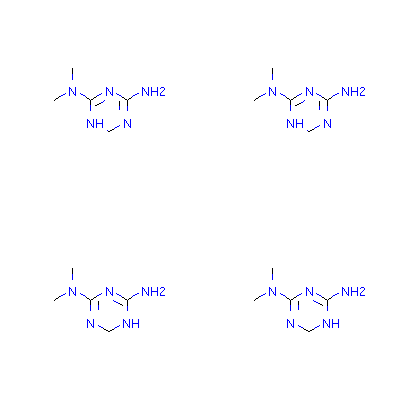
\includegraphics[scale=0.6]{triazineCA.png} & & [0.7]& [0.7] & [21] \\
\hline
27 & tetrazole & 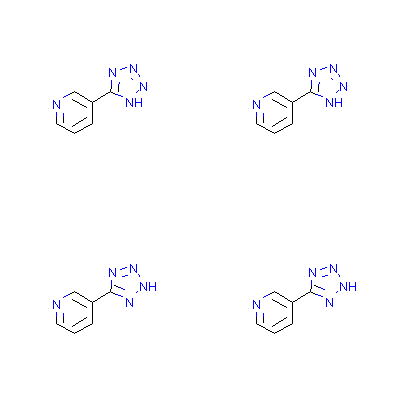
\includegraphics[scale=0.6]{tetrazoleCA.png} & & [1.0]& [0.73] & [22] \\
\hline
28 & phenol & 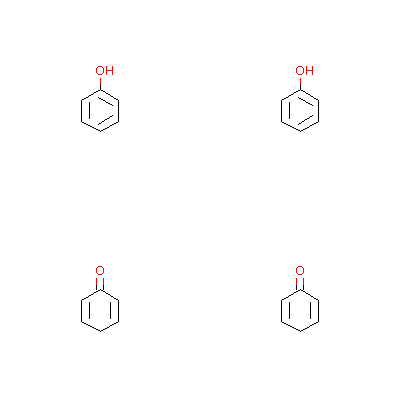
\includegraphics[scale=0.6]{phenolCA.png} & & [0.4]& [0.25] & [68] \\
\hline
29 & phosphor & 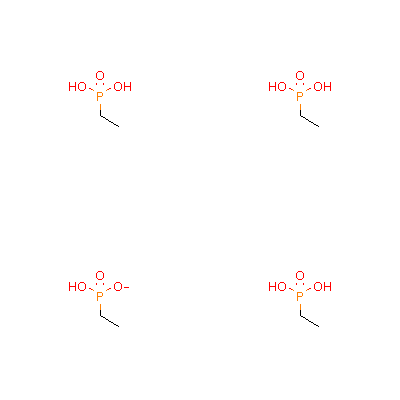
\includegraphics[scale=0.6]{phosphorCA.png} & & [1.0]& [1.0] & [0] \\
\hline
30 & 112and113 & 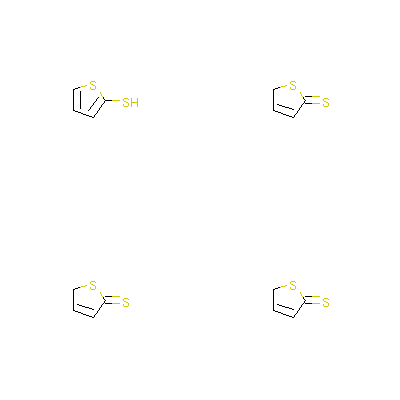
\includegraphics[scale=0.6]{112and113CA.png} & & [1.0]& [1.0] & [0] \\
\hline
31 & NO & 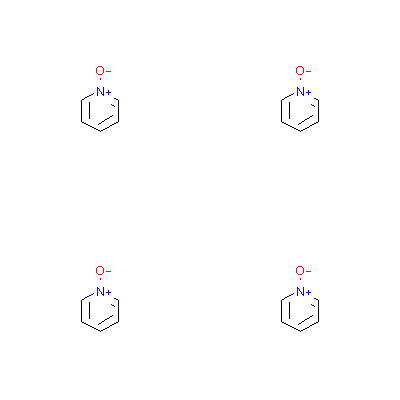
\includegraphics[scale=0.6]{NOCA.png} & & [1.0]& [1.0] & [0] \\
\hline
32 & diazo & 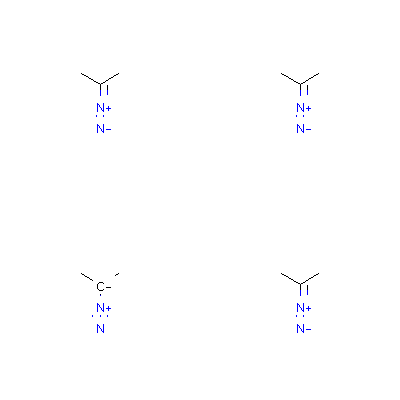
\includegraphics[scale=0.6]{diazoCA.png} & & [1.0]& [1.0] & [0] \\
\hline
33 & benzaldoxime & 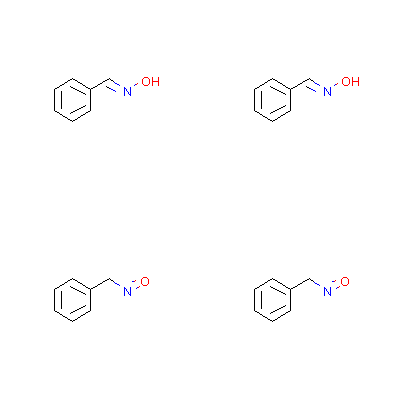
\includegraphics[scale=0.6]{benzaldoximeCA.png} & & [0.57]& [0.58] & [55] \\
\hline
34 & quatAmMesomer3 & 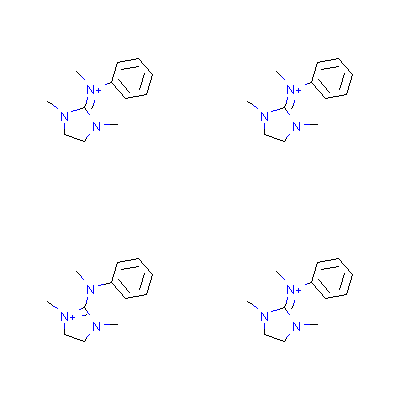
\includegraphics[scale=0.6]{quatAmMesomer3CA.png} & & [1.0]& [1.0] & [0] \\
\hline
35 & NNO & 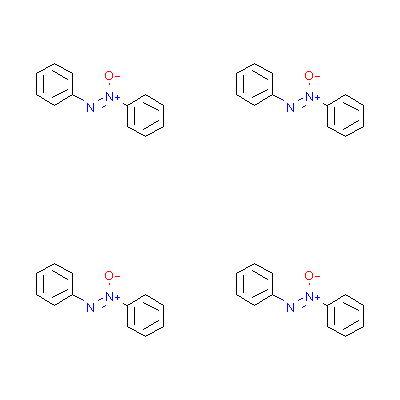
\includegraphics[scale=0.6]{NNOCA.png} & & [1.0]& [1.0] & [0] \\
\hline
36 & amide & 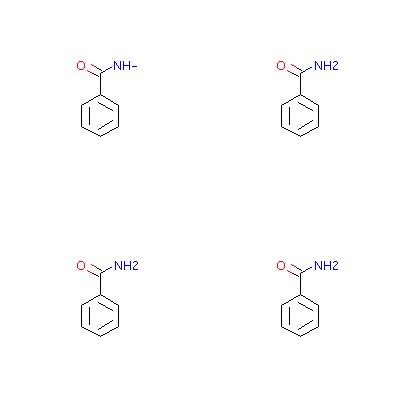
\includegraphics[scale=0.6]{amideCA.png} & & [1.0]& [1.0] & [0] \\
\hline
37 & thiopurine & 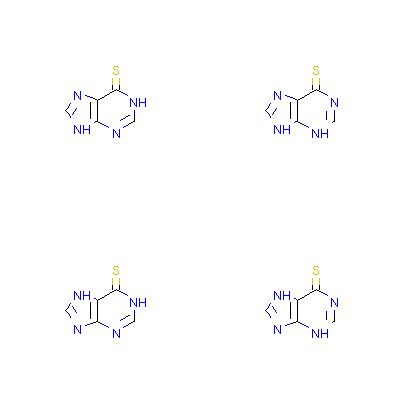
\includegraphics[scale=0.6]{thiopurineCA.png} & & [1.0]& [0.72] & [21] \\
\hline
\end{longtable}
\end{landscape}

\section{Additional standardization with MolVS}

In addition to running Standardizer by ChemAxon, the canonicalize and uncharge options of MolVS were used.

\begin{landscape}
\begin{longtable}{|l|l|l|l|l|l|l|}
\hline
Idx & Name & Structure In and Out & Comment & TanTop & DiceMorgan & No. of DescDiff\\
\hline
1 & clopidol & 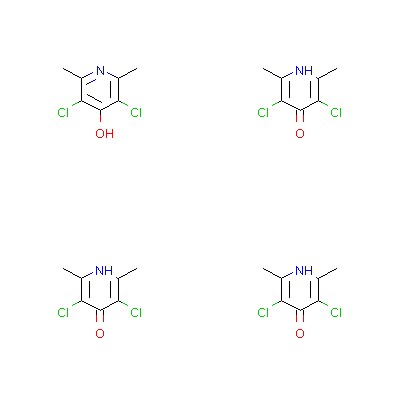
\includegraphics[scale=0.6]{clopidolMV.png} & & [1.0]& [1.0] & [0] \\
\hline
2 & phthalimide & 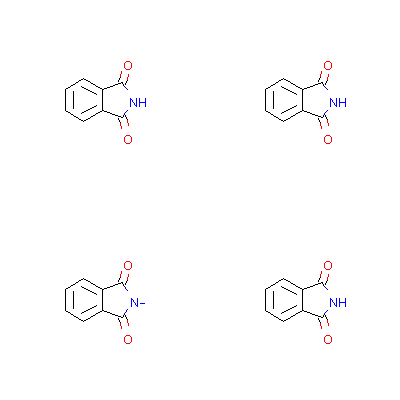
\includegraphics[scale=0.6]{phthalimideMV.png} & & [1.0]& [1.0] & [0] \\
\hline
3 & Viagra & 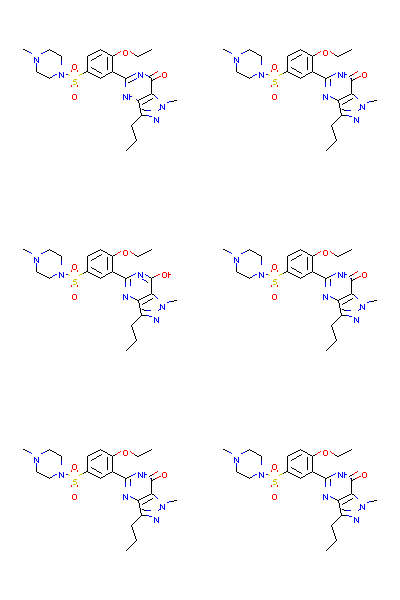
\includegraphics[scale=0.6]{ViagraMV.png} & & [1.0, 1.0, 1.0]& [1.0, 1.0, 1.0] & [0, 0, 0] \\
\hline
4 & quatAmMesomer & 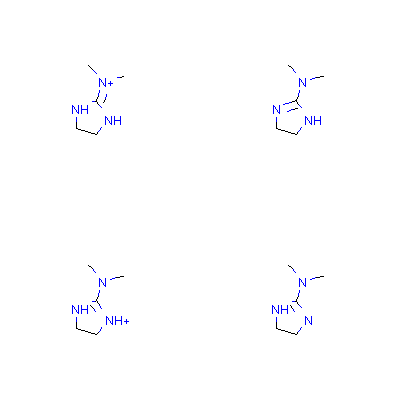
\includegraphics[scale=0.6]{quatAmMesomerMV.png} & & [1.0]& [1.0] & [1] \\
\hline
5 & pyridinol & 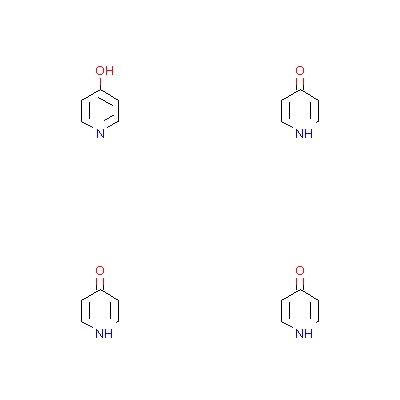
\includegraphics[scale=0.6]{pyridinolMV.png} & & [1.0]& [1.0] & [0] \\
\hline
6 & quatAmMesomer4 & 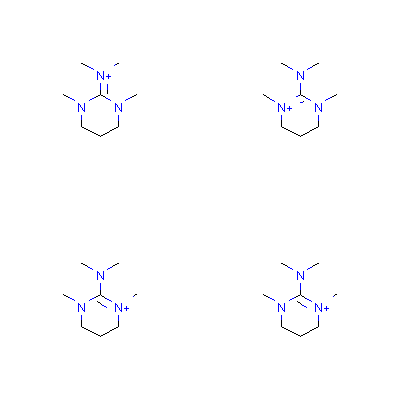
\includegraphics[scale=0.6]{quatAmMesomer4MV.png} & & [1.0]& [1.0] & [1] \\
\hline
7 & azide & 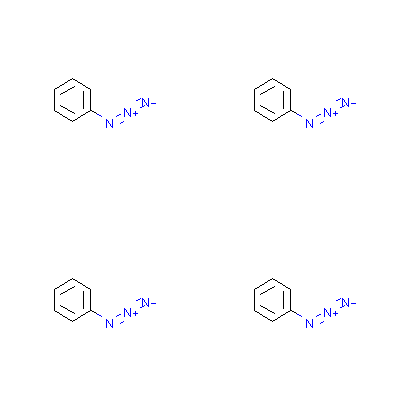
\includegraphics[scale=0.6]{azideMV.png} & & [1.0]& [1.0] & [0] \\
\hline
8 & triazinol & 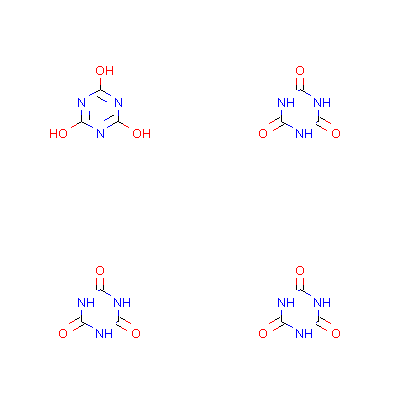
\includegraphics[scale=0.6]{triazinolMV.png} & & [1.0]& [1.0] & [0] \\
\hline
9 & phosphate & 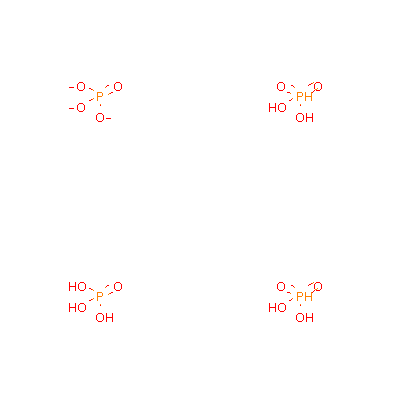
\includegraphics[scale=0.6]{phosphateMV.png} & & [1.0]& [1.0] & [0] \\
\hline
10 & Propenol & 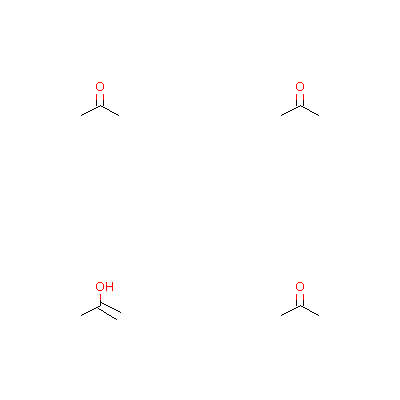
\includegraphics[scale=0.6]{PropenolMV.png} & & [1.0]& [1.0] & [0] \\
\hline
11 & phosphine & 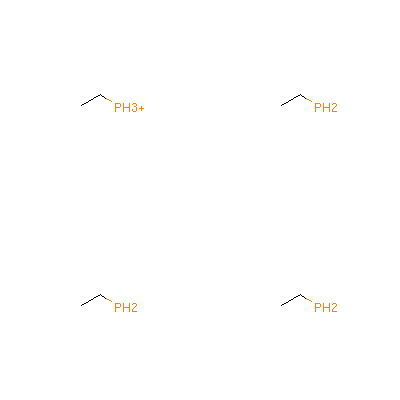
\includegraphics[scale=0.6]{phosphineMV.png} & & [1.0]& [1.0] & [0] \\
\hline
12 & cicletanine & 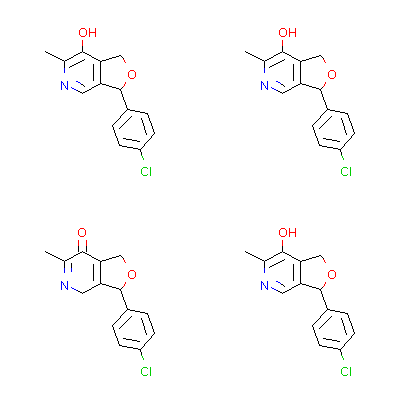
\includegraphics[scale=0.6]{cicletanineMV.png} & & [1.0]& [1.0] & [0] \\
\hline
13 & propaneAcid & \includegraphics[scale=0.6]{propaneAcidMV.png} & & [1.0]& [1.0] & [0] \\
\hline
14 & imidazole & \includegraphics[scale=0.6]{imidazoleMV.png} & & [1.0]& [1.0] & [0] \\
\hline
15 & enamine & \includegraphics[scale=0.6]{enamineMV.png} & & [1.0]& [1.0] & [0] \\
\hline
16 & sulfoxide & \includegraphics[scale=0.6]{sulfoxideMV.png} & & [1.0]& [1.0] & [0] \\
\hline
17 & sulfonamide & \includegraphics[scale=0.6]{sulfonamideMV.png} & & [1.0]& [1.0] & [0] \\
\hline
18 & tiouracil & \includegraphics[scale=0.6]{tiouracilMV.png} & & [1.0, 1.0, 1.0, 1.0, 1.0, 1.0]& [1.0, 1.0, 1.0, 1.0, 1.0, 1.0] & [0, 0, 0, 0, 0, 0] \\
\hline
19 & quatAmMesomer2 & \includegraphics[scale=0.6]{quatAmMesomer2MV.png} & & [1.0]& [1.0] & [0] \\
\hline
20 & nitro & \includegraphics[scale=0.6]{nitroMV.png} & & [0.67, 1.0, 0.67]& [0.56, 0.8, 0.6] & [58, 43, 56] \\
\hline
21 & 107and108and109 & \includegraphics[scale=0.6]{107and108and109MV.png} & & [1.0, 1.0, 1.0]& [1.0, 1.0, 1.0] & [0, 0, 0] \\
\hline
22 & aminopyrimidine & \includegraphics[scale=0.6]{aminopyrimidineMV.png} & & [1.0]& [1.0] & [0] \\
\hline
23 & 105and106 & \includegraphics[scale=0.6]{105and106MV.png} & & [1.0]& [1.0] & [0] \\
\hline
24 & Rhodamine & \includegraphics[scale=0.6]{RhodamineMV.png} & & [1.0]& [1.0] & [0] \\
\hline
25 & sulfon & \includegraphics[scale=0.6]{sulfonMV.png} & & [1.0]& [1.0] & [0] \\
\hline
26 & triazine & \includegraphics[scale=0.6]{triazineMV.png} & & [1.0]& [1.0] & [0] \\
\hline
27 & tetrazole & \includegraphics[scale=0.6]{tetrazoleMV.png} & & [1.0]& [1.0] & [1] \\
\hline
28 & phenol & \includegraphics[scale=0.6]{phenolMV.png} & & [1.0]& [1.0] & [0] \\
\hline
29 & phosphor & \includegraphics[scale=0.6]{phosphorMV.png} & & [1.0]& [1.0] & [0] \\
\hline
30 & 112and113 & \includegraphics[scale=0.6]{112and113MV.png} & & [1.0]& [1.0] & [0] \\
\hline
31 & NO & \includegraphics[scale=0.6]{NOMV.png} & & [1.0]& [1.0] & [0] \\
\hline
32 & diazo & \includegraphics[scale=0.6]{diazoMV.png} & & [1.0]& [1.0] & [0] \\
\hline
33 & benzaldoxime & \includegraphics[scale=0.6]{benzaldoximeMV.png} & & [1.0]& [1.0] & [0] \\
\hline
34 & quatAmMesomer3 & \includegraphics[scale=0.6]{quatAmMesomer3MV.png} & & [1.0]& [1.0] & [0] \\
\hline
35 & NNO & \includegraphics[scale=0.6]{NNOMV.png} & & [1.0]& [1.0] & [0] \\
\hline
36 & amide & \includegraphics[scale=0.6]{amideMV.png} & & [1.0]& [1.0] & [0] \\
\hline
37 & thiopurine & \includegraphics[scale=0.6]{thiopurineMV.png} & & [1.0]& [1.0] & [0] \\
\hline
\end{longtable}
\end{landscape}

\end{document}
